\documentclass[12pt]{scrartcl}

\usepackage{amsmath,amssymb}
\usepackage{fullpage}
\usepackage{enumitem}
\usepackage{hyperref}
\usepackage{graphicx}
\usepackage{tikz}
\usepackage{pgfplots}
\usepackage{float}
\usepackage{tabularx}
\usepackage{titlesec}

\pgfplotsset{compat=1.18}
\usetikzlibrary{trees,positioning,shapes,arrows,shadows}
\usepgfplotslibrary{statistics,groupplots} 
\setlength{\parindent}{0pt}

\tikzset{
  basic/.style  = {draw, text width=2cm, drop shadow, font=\sffamily, rectangle},
  root/.style   = {basic, rounded corners=2pt, thin, align=center, fill=white},
  level-2/.style = {basic, rounded corners=6pt, thin,align=center, fill=white, text width=4cm},
  level-3/.style = {basic, thin, align=center, fill=white, text width=3cm}
}

\titleformat{\section}  % which section command to format
{\fontsize{12}{14}\bfseries} % format for whole line
{\thesection} % how to show number
{1em} % space between number and text
{} % formatting for just the text
[] % formatting for after the text

\titleformat{\subsection}  % which section command to format
{\fontsize{12}{14}\bfseries} % format for whole line
{\thesubsection} % how to show number
{1em} % space between number and text
{} % formatting for just the text
[] % formatting for after the text

\begin{document}

\begin{center}
	\hrule
	\vspace{0.4cm}
	{\textbf{\large Lecture 05: Sampling and Sampling Distributions}} \\ [0.2cm]
	INF1004 Mathematics II

\end{center}

\textbf{Name:} Timothy Chia \hspace{\fill} \textbf{Date:}  09/02/2026\\

\hrule

\section{The Framework of Statistical Studies}
Statistical inquiry begins with a curiosity about a population, yet in practice, it is rarely possible to measure every individual within that population. Instead, we rely on samples to provide the data necessary for inference. The validity of these inferences depends heavily on the design of the study. \\

We generally categorise studies into three types based on the level of intervention. \textbf{Descriptive research}, or a sample survey, involves collecting data through random sampling to describe characteristics without attempting to influence the subjects. \textbf{Observational studies} go a step further by observing individuals to learn about a group, but the researcher specifically avoids interfering with the subjects aside from measurement. While these studies are excellent for establishing correlation, they cannot establish causality because of potential confounding or lurking variables. To determine cause and effect, a \textbf{Randomised Controlled Experiment} is required. Here, the researcher deliberately imposes different treatments on different groups to observe how a specific response variable changes, allowing for the establishment of a causal link.

\begin{figure}[H]
    \centering
    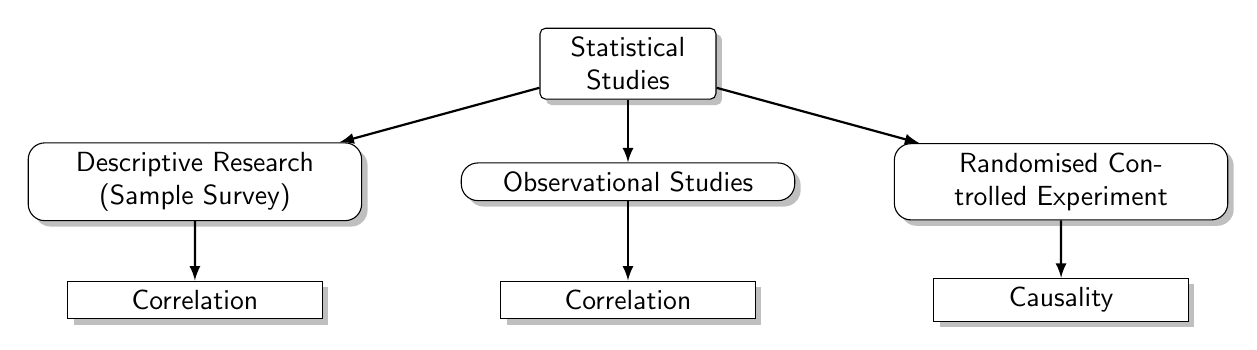
\begin{tikzpicture}[
        node distance=2.5cm,
        level 1/.style={sibling distance=5.5cm},
        level 2/.style={sibling distance=3.5cm},
        edge from parent/.style={draw, -latex, thick}
    ]
        \node [root] {Statistical Studies}
            child {node [level-2] {Descriptive Research\\(Sample Survey)}
                child {node [level-3] {Correlation}}
            }
            child {node [level-2] {Observational Studies}
                child {node [level-3] {Correlation}}
            }
            child {node [level-2] {Randomised Controlled Experiment}
                child {node [level-3] {Causality}}
            };
    \end{tikzpicture}
    \caption{Hierarchy of statistical studies and their ability to establish correlation versus causality.}
\end{figure}

\section{Methodologies for Data Collection}
The ``best'' way to sample is defined by the goal of obtaining a representative subset of the population that exhibits sufficient variability and high data quality. We distinguish between probability and non-probability sampling. \\

\textbf{Probability sampling} is the gold standard because it ensures that every member of the population has a known, non-zero chance of being selected. The most fundamental type is \textbf{Simple Random Sampling (SRS)}, where random numbers are used to ensure every individual has an equal probability of inclusion. \textbf{Systematic Sampling} simplifies this by choosing a random starting point and then selecting every $k$-th member at a constant interval. \\

For more complex populations, we use \textbf{Cluster Sampling} or \textbf{Stratified Sampling}. In cluster sampling, the population is divided into groups (clusters) that are ideally representative of the whole; one or more clusters are then randomly selected in their entirety. Conversely, stratified sampling is used when the population contains distinct subgroups, or strata (such as different income levels or academic majors). A simple random sample is taken from \textit{each} stratum, ensuring that even small subgroups are represented proportionally in the final sample. \\

In contrast, \textbf{Non-probability sampling} methods, such as \textbf{Convenience Sampling} (picking those who are easiest to reach) or \textbf{Self-selected/Voluntary Response Sampling}, often lead to biased results. These methods typically attract individuals with strong opinions or specific characteristics, rendering the resulting data statistically meaningless for population inference.

\begin{figure}[H]
    \centering
    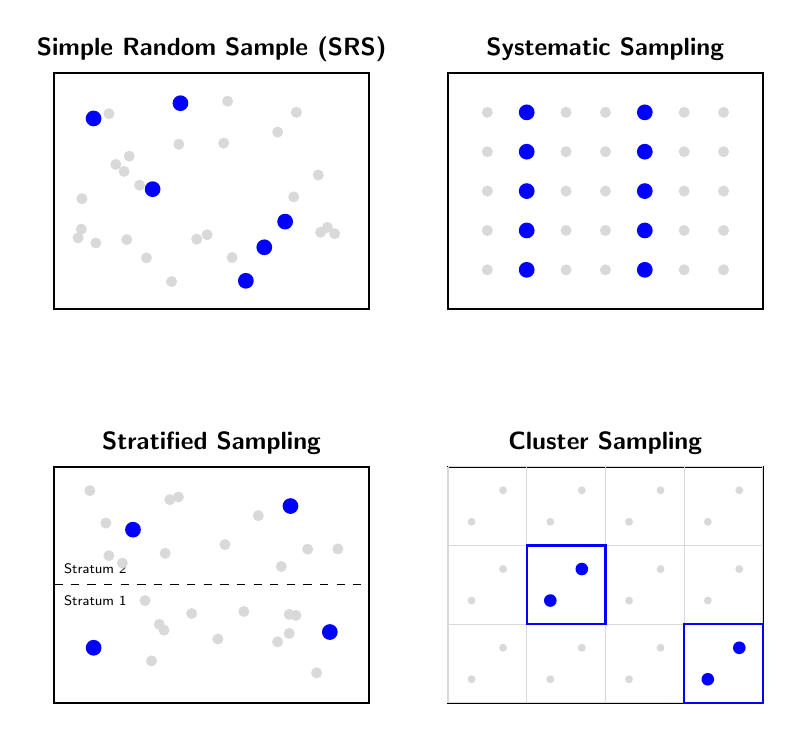
\begin{tikzpicture}[node distance=1cm, font=\sffamily\small]
        % SRS
        \begin{scope}[shift={(0,0)}]
            \draw[thick] (0,0) rectangle (4,3);
            \node at (2, 3.3) {\textbf{Simple Random Sample (SRS)}};
            \foreach \i in {1,...,25}
                \fill[gray!30] (0.3+3.4*rnd, 0.3+2.4*rnd) circle (0.07);
            \foreach \i in {1,...,6}
                \fill[blue] (0.3+3.4*rnd, 0.3+2.4*rnd) circle (0.1);
        \end{scope}
        
        % Systematic
        \begin{scope}[shift={(5,0)}]
            \draw[thick] (0,0) rectangle (4,3);
            \node at (2, 3.3) {\textbf{Systematic Sampling}};
            \foreach \x in {0.5, 1.0, ..., 3.5}
                \foreach \y in {0.5, 1.0, ..., 2.5}
                    \fill[gray!30] (\x, \y) circle (0.07);
            \foreach \y in {0.5, 1.0, ..., 2.5}
                \fill[blue] (1.0, \y) circle (0.1);
            \foreach \y in {0.5, 1.0, ..., 2.5}
                \fill[blue] (2.5, \y) circle (0.1);
        \end{scope}
        
        % Stratified
        \begin{scope}[shift={(0,-5)}]
            \draw[thick] (0,0) rectangle (4,3);
            \node at (2, 3.3) {\textbf{Stratified Sampling}};
            \draw[dashed] (0, 1.5) -- (4, 1.5);
            \node[anchor=west] at (0, 1.3) {\tiny Stratum 1};
            \node[anchor=west] at (0, 1.7) {\tiny Stratum 2};
            \foreach \i in {1,...,12} {
                \fill[gray!30] (0.3+3.4*rnd, 0.3+1.0*rnd) circle (0.07);
                \fill[gray!30] (0.3+3.4*rnd, 1.7+1.0*rnd) circle (0.07);
            }
            \fill[blue] (0.5, 0.7) circle (0.1);
            \fill[blue] (3.5, 0.9) circle (0.1);
            \fill[blue] (1.0, 2.2) circle (0.1);
            \fill[blue] (3.0, 2.5) circle (0.1);
        \end{scope}
        
        % Cluster
        \begin{scope}[shift={(5,-5)}]
            \draw[thick] (0,0) rectangle (4,3);
            \node at (2, 3.3) {\textbf{Cluster Sampling}};
            \draw[step=1cm, gray!30, thin] (0,0) grid (4,3);
            \foreach \x in {0.5, 1.5, 2.5, 3.5}
                \foreach \y in {0.5, 1.5, 2.5} {
                    \fill[gray!30] (\x-0.2, \y-0.2) circle (0.05);
                    \fill[gray!30] (\x+0.2, \y+0.2) circle (0.05);
                }
            % Select some clusters
            \draw[blue, thick] (1,1) rectangle (2,2);
            \fill[blue] (1.5-0.2, 1.5-0.2) circle (0.08);
            \fill[blue] (1.5+0.2, 1.5+0.2) circle (0.08);
            \draw[blue, thick] (3,0) rectangle (4,1);
            \fill[blue] (3.5-0.2, 0.5-0.2) circle (0.08);
            \fill[blue] (3.5+0.2, 0.5+0.2) circle (0.08);
        \end{scope}
    \end{tikzpicture}
    \caption{Comparison of probability sampling methods: Simple Random, Systematic, Stratified, and Cluster sampling.}
\end{figure}

\newpage
\section{The Logic of Statistical Inference}
The ultimate goal of sampling is to calculate a \textbf{sample statistic}---a summary number like the mean $\bar{x}$ or standard deviation $s$---and use it to infer a \textbf{population parameter}, such as the population mean $\mu$ or population standard deviation $\sigma$. \\

However, we must account for \textbf{sampling variability}. If we were to take multiple samples of the same size $n$ from the same population, the resulting statistics would vary from sample to sample. By treating the sample statistic as a random variable, we can construct a \textbf{sampling distribution}. This distribution represents the probability of all possible values the statistic could take. It is this distribution, rather than the distribution of the raw data itself, that allows us to quantify the uncertainty in our estimates and calculate the expected value and variance of our estimators.

\begin{figure}[H]
    \centering
    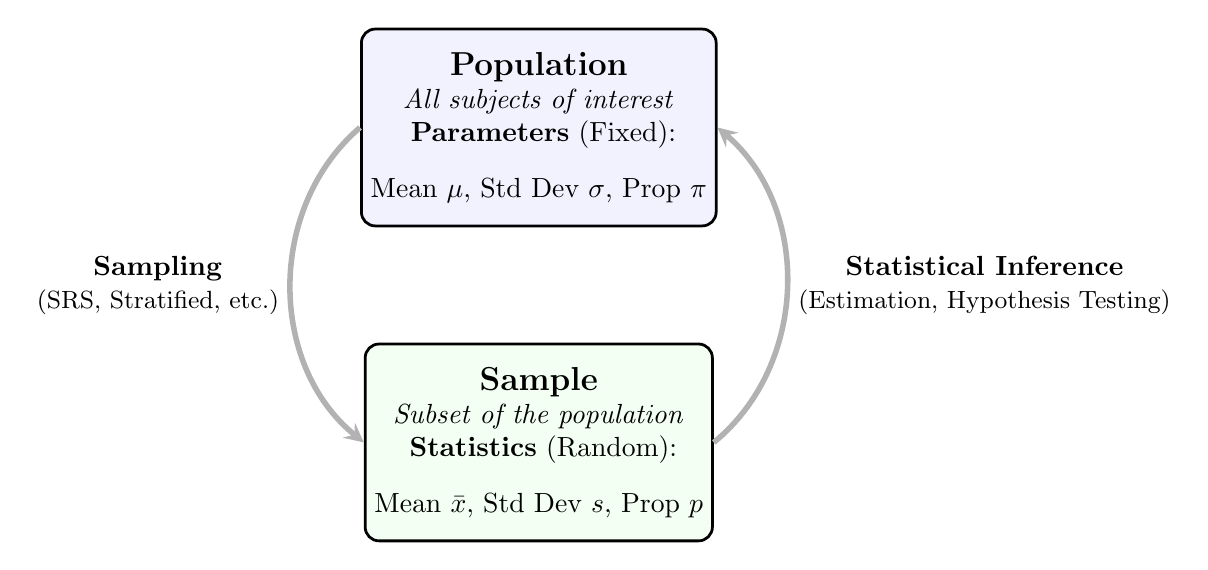
\begin{tikzpicture}[
        box/.style={draw, rectangle, rounded corners=5pt, minimum width=4cm, minimum height=2.5cm, align=center, fill=white, line width=1pt},
        arrow/.style={-stealth, line width=2pt, draw=gray!60}
    ]
        \node[box, fill=blue!5] (pop) at (0,4) {
            \textbf{\large Population} \\
            \textit{All subjects of interest} \\
            \vspace{0.2cm}
            \textbf{Parameters} (Fixed): \\
            Mean $\mu$, Std Dev $\sigma$, Prop $\pi$
        };
        
        \node[box, fill=green!5] (sam) at (0,0) {
            \textbf{\large Sample} \\
            \textit{Subset of the population} \\
            \vspace{0.2cm}
            \textbf{Statistics} (Random): \\
            Mean $\bar{x}$, Std Dev $s$, Prop $p$
        };
        
        \draw[arrow] (pop.west) to [bend right=50] node[midway, left, align=center, color=black] {
            \textbf{Sampling} \\
            \small (SRS, Stratified, etc.)
        } (sam.west);
        
        \draw[arrow] (sam.east) to [bend right=50] node[midway, right, align=center, color=black] {
            \textbf{Statistical Inference} \\
            \small (Estimation, Hypothesis Testing)
        } (pop.east);
    \end{tikzpicture}
    \caption{The cycle of statistical inference, showing the relationship between fixed population parameters and random sample statistics.}
\end{figure}

\section{The Central Limit Theorem (CLT)}
The Central Limit Theorem is the cornerstone of inferential statistics. It states that regardless of the shape of the original population distribution---whether it be normal, uniform, exponential, or parabolic---the sampling distribution of the sample mean $\bar{x}$ will approach a normal distribution as the sample size $n$ increases. \\

A common rule of thumb is that a sample size of $n \ge 30$ is ``sufficiently large'' for this approximation to hold. Under these conditions, the sampling distribution of the mean will have a mean equal to the population mean $\mu$ and a standard deviation, often called the \textbf{Standard Error (SE)}, defined by:

\[ \sigma_{\bar{x}} = \frac{\sigma}{\sqrt{n}} \]

To find the probability that a sample mean falls within a certain range, we convert the sample mean into standard units using the Z-score formula for means:

\[ Z = \frac{\bar{x} - \mu}{\sigma / \sqrt{n}} \]

\begin{figure}[H]
    \centering
    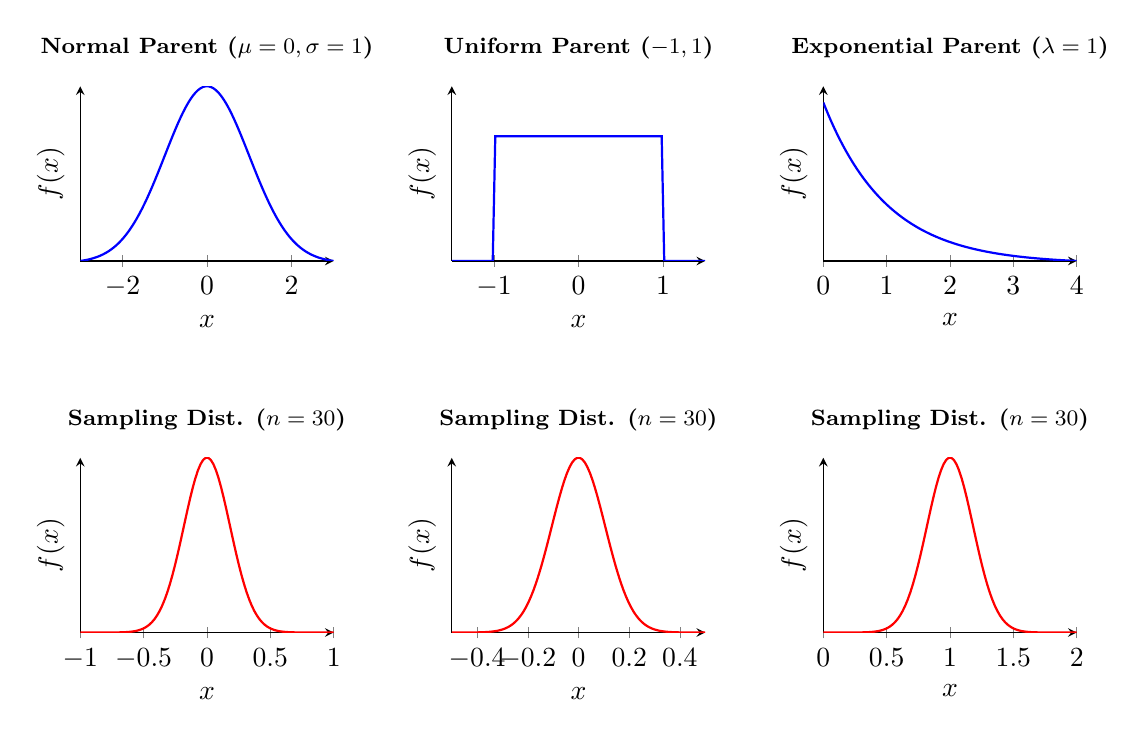
\begin{tikzpicture}
        \begin{groupplot}[
            group style={
                group size=3 by 2,
                vertical sep=2.5cm,
                horizontal sep=1.5cm
            },
            width=4.8cm,
            height=3.8cm,
            samples=100,
            no markers,
            xlabel={$x$},
            ylabel={$f(x)$},
            every axis title/.style={at={(0.5,1.1)}, anchor=south, font=\footnotesize\bfseries},
            axis lines=left,
            enlarge x limits=false,
            ytick=\empty
        ]
            % Row 1: Parent Distributions
            \nextgroupplot[title={Normal Parent ($\mu=0, \sigma=1$)}, domain=-3:3]
            \addplot[blue, thick] {exp(-0.5*x^2)/sqrt(2*pi)};
            
            \nextgroupplot[title={Uniform Parent ($-1, 1$)}, domain=-1.5:1.5, ymax=0.7]
            \addplot[blue, thick] {abs(x)<=1 ? 0.5 : 0};
            
            \nextgroupplot[title={Exponential Parent ($\lambda=1$)}, domain=0:4, ymax=1.1]
            \addplot[blue, thick] {exp(-x)};
            
            % Row 2: Sampling Distributions (n=30)
            \nextgroupplot[title={Sampling Dist. ($n=30$)}, domain=-1:1]
            \addplot[red, thick] {exp(-15*x^2) / 0.4576};
            
            \nextgroupplot[title={Sampling Dist. ($n=30$)}, domain=-0.5:0.5]
            \addplot[red, thick] {exp(-45*x^2) / 0.2642};
            
            \nextgroupplot[title={Sampling Dist. ($n=30$)}, domain=0:2]
            \addplot[red, thick] {exp(-15*(x-1)^2) / 0.4576};
        \end{groupplot}
    \end{tikzpicture}
    \caption{Convergence of the sampling distribution of the mean toward a normal distribution as $n$ increases, regardless of the parent population's shape.}
\end{figure}

\section{Inference for Smaller Samples and the T-Distribution}
In many real-world scenarios, we encounter two significant hurdles: our sample size is small ($n < 30$), and we do not know the true population standard deviation $\sigma$. In these cases, using the Z-distribution is inappropriate because it tends to underestimate the variability in small samples when the sample standard deviation $s$ is used as a proxy for $\sigma$. \\

Instead, we employ \textbf{Student's t-distribution}. This distribution is similar in shape to the normal distribution but has ``fatter tails'', which accounts for the extra uncertainty introduced by estimating $\sigma$ with the sample standard deviation $s$. The t-distribution is a family of distributions defined by \textbf{degrees of freedom ($df$)}, where:

\[ df = n - 1 \]

The concept of degrees of freedom refers to the number of variables in the sample that are free to vary. For example, if a sample $\{a, b, c\}$ has a known mean of 2, once the values of $a$ and $b$ are chosen, the value of $c$ is fixed. Thus, only $n-1$ values are truly ``free.'' As the degrees of freedom increase, the t-distribution becomes narrower and eventually converges with the standard normal distribution. The statistic used for this model is:

\[ t = \frac{\bar{x} - \mu}{s / \sqrt{n}} \]

\begin{figure}[H]
    \centering
    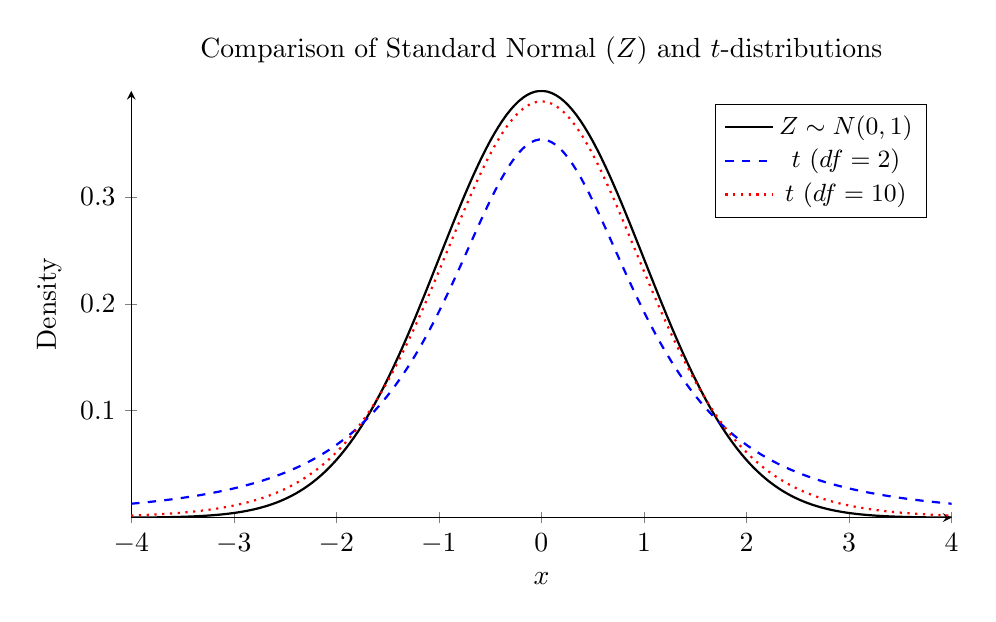
\begin{tikzpicture}
        \begin{axis}[
            width=12cm,
            height=7cm,
            samples=200,
            no markers,
            domain=-4:4,
            axis lines=left,
            xlabel={$x$},
            ylabel={Density},
            legend pos=north east,
            legend style={font=\small},
            title={Comparison of Standard Normal ($Z$) and $t$-distributions},
            enlarge x limits=false
        ]
            \addplot[black, thick] {exp(-0.5*x^2)/sqrt(2*pi)};
            \addlegendentry{$Z \sim N(0,1)$}
            
            \addplot[blue, thick, dashed] {(1+x^2/2)^(-1.5) * 0.3536};
            \addlegendentry{$t$ ($df=2$)}
            
            \addplot[red, thick, dotted] {(1+x^2/10)^(-5.5) * 0.3891};
            \addlegendentry{$t$ ($df=10$)}
        \end{axis}
    \end{tikzpicture}
    \caption{The $t$-distribution has heavier tails and a lower peak for smaller degrees of freedom ($df$), providing a more conservative model for small samples. As $df$ increases, it approaches the standard normal distribution.}
\end{figure}

\end{document}
